\documentclass{beamer}

\mode<presentation>
{
  \usetheme{default}
  \usecolortheme{default}
  \usefonttheme{default}
  \setbeamertemplate{navigation symbols}{}
  \setbeamertemplate{caption}[numbered]
  \setbeamertemplate{footline}[page number]
  \setbeamercolor{frametitle}{fg=white}
  \setbeamercolor{footline}{fg=black}
} 

\usepackage[english]{babel}
\usepackage[utf8x]{inputenc}
\usepackage{tikz}
\usepackage{listings}
\usepackage{courier}
\usepackage{array}
\usepackage{bold-extra}
\usepackage{minted}
\usepackage{dirtree}

\xdefinecolor{darkblue}{rgb}{0.1,0.1,0.7}
\xdefinecolor{darkgreen}{rgb}{0,0.5,0}
\xdefinecolor{darkgrey}{rgb}{0.35,0.35,0.35}
\xdefinecolor{darkorange}{rgb}{0.8,0.5,0}
\xdefinecolor{darkred}{rgb}{0.7,0,0}
\xdefinecolor{dianablue}{rgb}{0.18,0.24,0.31}
\definecolor{commentgreen}{rgb}{0,0.6,0}
\definecolor{stringmauve}{rgb}{0.58,0,0.82}

\lstset{ %
  backgroundcolor=\color{white},      % choose the background color
  basicstyle=\ttfamily\small,         % size of fonts used for the code
  breaklines=true,                    % automatic line breaking only at whitespace
  captionpos=b,                       % sets the caption-position to bottom
  commentstyle=\color{commentgreen},  % comment style
  escapeinside={\%*}{*)},             % if you want to add LaTeX within your code
  keywordstyle=\color{blue},          % keyword style
  stringstyle=\color{stringmauve},    % string literal style
  showstringspaces=false,
  showlines=true
}

\lstdefinelanguage{scala}{
  morekeywords={abstract,case,catch,class,def,%
    do,else,extends,false,final,finally,%
    for,if,implicit,import,match,mixin,%
    new,null,object,override,package,%
    private,protected,requires,return,sealed,%
    super,this,throw,trait,true,try,%
    type,val,var,while,with,yield},
  otherkeywords={=>,<-,<\%,<:,>:,\#,@},
  sensitive=true,
  morecomment=[l]{//},
  morecomment=[n]{/*}{*/},
  morestring=[b]",
  morestring=[b]',
  morestring=[b]"""
}

\title[2016-12-21-femtocode-odg]{Declarative query language for deeply nested data}
\author{Jim Pivarski}
\institute{Princeton University -- DIANA}
\date{December, 21, 2016}

\begin{document}

\logo{\pgfputat{\pgfxy(0.11, 8)}{\pgfbox[right,base]{\tikz{\filldraw[fill=dianablue, draw=none] (0 cm, 0 cm) rectangle (50 cm, 1 cm);}}}\pgfputat{\pgfxy(0.11, -0.6)}{\pgfbox[right,base]{\tikz{\filldraw[fill=dianablue, draw=none] (0 cm, 0 cm) rectangle (50 cm, 1 cm);}\tikz{\filldraw[fill=dianablue, draw=none] (0 cm, 0 cm) rectangle (4.9 cm, 1 cm);}}}}

\begin{frame}
  \titlepage
\end{frame}

\logo{\pgfputat{\pgfxy(0.11, 8)}{\pgfbox[right,base]{\tikz{\filldraw[fill=dianablue, draw=none] (0 cm, 0 cm) rectangle (50 cm, 1 cm);}}}}

% Uncomment these lines for an automatically generated outline.
%\begin{frame}{Outline}
%  \tableofcontents
%\end{frame}

%%%%%%%%%%%%%%%%%%%%%%%%%%%%%%%%%%%%%%%%%%%%%%%%%%%%%%%

\begin{frame}{I've been thinking about computational speed recently}
\vspace{0.5 cm}
\begin{itemize}\setlength{\itemsep}{0.5 cm}
\item Physicists have been thinking about single-processor efficiency for decades, and are now thinking about scale-out.
\item Big Data community has been thinking about scale-out since it began, and is now thinking about single-processor \mbox{efficiency.\hspace{-1 cm}}
\vspace{0.25 cm}
\begin{itemize}\setlength{\itemsep}{0.1 cm}
\item Spark's Catalyst optimizer and Project Tungsten
\item Ibis, Impala, Kudu, Dremel/Drill\ldots
\end{itemize}
\item \textcolor{darkblue}{Speed is not a luxury:} the time between a query and its response limits a human data analyst's ability to develop instinct and see larger relationships.

\vspace{0.5 cm}
\textcolor{gray}{\it ``Answers can change the question line\ldots\ every time.''}

\mbox{ } \hfill \textcolor{gray}{--- Adam Ant}
\end{itemize}
\end{frame}

\begin{frame}{Hurdle Theory}
\vspace{0.5 cm}
\textcolor{darkblue}{My favorite metaphor for computational speed:} fast software is not like a fast runner, who has some superior intrinsic ability. All programs run at the same rate, the clock rate. But some have more hurdles on the track than others.

\vspace{0.25 cm}
\begin{center}
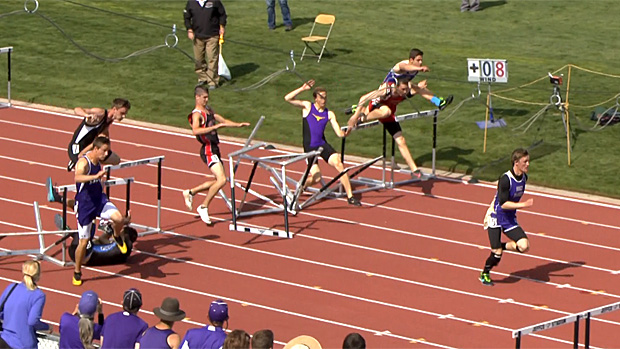
\includegraphics[width=0.7\linewidth]{hurdle9.jpg}
\end{center}
\end{frame}

\begin{frame}{But it's more than that\ldots}
\vspace{0.5 cm}
\begin{columns}
\column{0.4\linewidth}
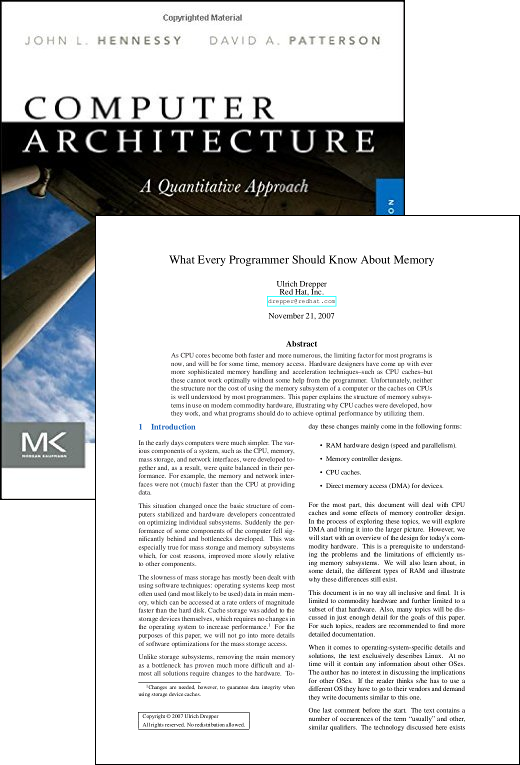
\includegraphics[width=\linewidth]{books.png}

\column{0.55\linewidth}
\textcolor{darkblue}{Gotcha: many of these hurdles are invisible!}

\vspace{0.5 cm}
Since the 90's, improvements in processor speed have outpaced improvements in memory bandwidth, so now memory is the bottleneck.

\vspace{0.5 cm}
Also, slow operations are pipelined to optimize throughput: many clock ticks from start to finish, but a full pipeline can finalize an operation in each clock tick.

\vspace{0.5 cm}
``Bubbles'' in the pipeline \mbox{thwart this.\hspace{-1 cm}}
\end{columns}
\end{frame}

\begin{frame}[fragile]{What fast code looks like}
\vspace{0.5 cm}
\begin{center}
\begin{minipage}{0.85\linewidth}
\begin{minted}[frame=single]{c++}
for (int i = 0;  i < huge_number;  i++)
  out[i] = in1[i] / in2[i];
\end{minted}
\end{minipage}
\end{center}

\begin{itemize}\setlength{\itemsep}{0.25 cm}
\item Simple loop structure that the compiler can unfold.
\item Forward stride that the CPU can detect and prefetch memory. (Arrays are contiguous in memory and should be properly aligned. Bonus points if you can {\tt \_\_restrict\_\_} aliasing.)
\item Bubble-free pipeline (except at start and end; edge effects).
\item Would allow SIMD parallelism that could be vectorized \\ (1024 at once in a GPU, 4 or 8 for MMX, 256 for KNL\ldots).
\end{itemize}
\end{frame}

\begin{frame}{Field is ripe with low-hanging fruit}
\vspace{0.5 cm}
\textcolor{darkblue}{I've estimated that our weeks-long physics jobs, which touch hundreds of terabytes, could be reduced to minutes or seconds.}
\begin{itemize}
\item Only need to touch $\sim$80~GB of {\it columnar} data in typical 100~million event query.
\item {\it Single} processor can load 80~GB data arrays in 20~minutes \\ (so divide by $N$, number of processors).
\item Optimized C++ code can perform one simple operation in 12~seconds. (Divide by $N$ and cache in memory.)
\item Low-end GPU can perform the same operation in 5~seconds. 12 seconds to copy over. (Divide by $N$ and cache on GPU.)
\end{itemize}

\vspace{0.5 cm}
\small
\textcolor{gray}{Actually a change in user behavior: ``weeks'' are spent making private skims to perform these operations quickly offline. But a shared server with sufficient caching would allow users to calculate one plot at a time, reducing the amount of data that needs to be read/copied.}
\end{frame}

\begin{frame}{Columns are essential}
\vspace{-1.5 cm}
\begin{itemize}\setlength{\itemsep}{0.25 cm}
\item Spark's Catalyst (SQL optimizations) and Project Tungsten (memory management) derive their benefit from columnar data and JIT-compilation.
\item \begin{minipage}[t]{0.5\linewidth}Even complex data structures can be represented as columns (``shredded'').\end{minipage}
\item \begin{minipage}[t]{0.5\linewidth}Mostly used to minimize disk access in file formats.\end{minipage}

\vspace{0.1 cm}
\begin{itemize}
\item Google Dremel
\item Apache Parquet
\item ROOT \textcolor{gray}{(physics, since 90's, unacknowledged in Google paper!)}
\end{itemize}

\item Modern SQL engines are actually executing code on the raw columns, rather than reconstructing records.
\end{itemize}

\vspace{-5 cm}
\mbox{ } \hfill 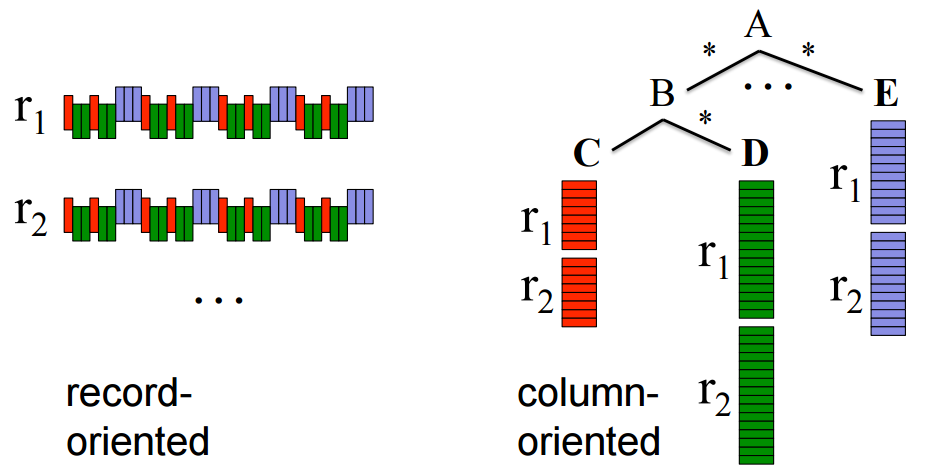
\includegraphics[width=0.4\linewidth]{columnar.png}
\end{frame}

\begin{frame}{But SQL is not expressive enough}
\vspace{0.5 cm}
\textcolor{darkblue}{Big irony:} modern DataFrames allow nested structure with clever shredding algorithms to work directly with raw columns, but the SQL language doesn't offer much for working with that structure.

\vspace{0.5 cm}
We discovered this while porting physics analyses to Spark: data are in DataFrames, but we can't do anything useful with them without dropping to RDDs.

\vspace{0.5 cm}
\begin{itemize}
\item RDD access is ten times slower.
\item Spark can't analyze black-box Scala or Python functions into work-plans.
\item Records must be reconstructed from columns to feed the functions.
\end{itemize}
\end{frame}

\begin{frame}[fragile]{Example: nested query in C (physics status quo)}
\vspace{0.25 cm}
\begin{center}
\begin{minipage}{0.95\linewidth}
\textcolor{darkblue}{``Momentum of the track with $|\eta|$ $<$ 2.4 that has the most hits.''}

\vspace{-0.5 cm}
\textcolor{darkblue}{\dirtree{%
.1 events.
.2 tracks.
.3 hits.
}}

\end{minipage}
\end{center}
\small
\begin{minted}[frame=single]{c++}
Track *best = NULL;
for (int i = 0;  i < tracks.size();  i++) {
  if (fabs(tracks[i]->eta) < 2.4)
    if (best == NULL ||
        tracks[i]->hits.size() > best->hits.size())
      best = tracks[i];
}
if (best != NULL)
  return best->pt;
else
  return 0.0;
\end{minted}

\vspace{-0.1 cm}
\textcolor{gray}{(DNS queries also have nested structure; wanted: other domain-specific examples.)}
\end{frame}

\begin{frame}[fragile]{Example: nested query in SQL}
\vspace{0.25 cm}
\begin{center}
\begin{minipage}{0.95\linewidth}
\textcolor{darkblue}{``Momentum of the track with $|\eta|$ $<$ 2.4 that has the most hits.''}
\end{minipage}
\end{center}
\small
\begin{minted}[frame=single]{sql}
WITH hit_stats AS (
  SELECT hit.track_id, COUNT(*) AS hit_count
    FROM hit GROUP BY hit.track_id),
 track_sorted AS (
    SELECT track.*, 
    ROW_NUMBER() OVER (
     PARTITION BY track.event_id
     ORDER BY hit_stats.hit_count DESC)
  track_ordinal FROM track INNER JOIN hit_stats
    ON hit_stats.track_id = track.id
    WHERE ABS(track.eta) < 2.4)
 SELECT * FROM event INNER JOIN track_sorted
   ON track_sorted.event_id = event.id
WHERE
  track_sorted.track_ordinal = 1
\end{minted}
\end{frame}

\begin{frame}[fragile]{Example: what it ought to look like}
\vspace{0.25 cm}
\begin{center}
\begin{minipage}{0.95\linewidth}
\textcolor{darkblue}{``Momentum of the track with $|\eta|$ $<$ 2.4 that has the most hits.''}
\end{minipage}
\end{center}
\small
\begin{onlyenv}<1>
\begin{minted}[frame=single]{bash}
tracks.filter(t => abs(t.eta) < 2.4) # drop tracks
      .maxBy(t => t.hits.size) # pick one (if any)
      .map(t => t.pt)          # transform it
      .impute(0.0)             # replace "None"
                               # with a value
\end{minted}
\end{onlyenv}
\begin{onlyenv}<2>
\begin{minted}[frame=single]{bash}
tracks.filter(abs($1.eta) < 2.4)     # drop tracks
      .maxBy($1.hits.size)     # pick one (if any)
      .map($1.pt)              # transform it
      .impute(0.0)             # replace "None"
                               # with a value
\end{minted}
\end{onlyenv}
\end{frame}

\begin{frame}{Summary}
\begin{description}
\item[SQL] is good at exploding data, but doesn't provide any support for rolling up transformed sublists. User has to create indexes and do ``joins'' (probably with a performance penalty).
\item[Scala/C++] can do anything, but performance is completely up to the user. The system can't examine a loop over events and rewrite it into vectorized operations on columns.
\item[Femtocode] is designed for this niche.
\end{description}
\end{frame}

\begin{frame}[fragile]{Femtocode is a unique language}
\vspace{0.25 cm}
\begin{itemize}
\item Provides an event-based, functional view of computation on identically typed, deeply structured data.
\item Rearranges the user's program to perform calculations on one columnar array at a time.
\end{itemize}

\begin{minted}[frame=single]{scala}
tracks.map(t => sqrt(t.px**2 + t.py**2)).max
\end{minted}

becomes

\vspace{-0.25 cm}
\begin{verbatim}
    @1 := .sqr(tracks.px)
    @2 := .sqr(tracks.py)
    @3 := +(@1, @2)
    @4 := sqrt(@3)
    @5 := .reduce.max(@4, tracks@size)
\end{verbatim}

where all of the above are implicit loops over arrays ({\tt @5} has one entry per event; the rest may have more).
\end{frame}

\begin{frame}{Attributes of Femtocode, to make this possible}
\vspace{0.25 cm}
\begin{description}
\item[Declarative:] order written/order evaluated are often not the same.
\item[Functional:] map/filter/maxBy say less than explicit ``for'' loops.
\item[Vectorized:] operations on rows (e.g.\ events) transformed by compiler into operations on columns.

\item[No unbounded loops:] number of steps in each operation is finite and determined by the input data.

\item[No runtime errors:] any compileable query will return some result.

\item[Statically typed:] stronger type system than most languages is needed to eliminate runtime errors.

\item[Second-class functions:] functions may be partly passed as objects, but must be known at compile-time (same as PFA).

\item[No recursion/not Turing complete:] consequence of no unbounded loops. Femtocode belongs to a small class of ``total functional'' languages.
\end{description}
\end{frame}

\begin{frame}{Comparison to PFA}
\vspace{0.3 cm}
\begin{columns}[t]
\column{0.5\linewidth}
\textcolor{darkblue}{\underline{The same}}

\begin{itemize}
\item Limited language, focused on math, must be fed data from outside.

\item ``Two language solution:'' restricted PFA/Femtocode controlled by Scala/Python in quoted blocks \textcolor{gray}{(like SQL)}.

\item ``Second class functions'' with the same limitations.

\item Multiple execution engines adhering to a common standard.

\item Intermediate representation is JSON.
\end{itemize}

\column{0.5\linewidth}
\textcolor{darkblue}{\underline{Different}}

\begin{itemize}
\item Total functional and fully vectorizable.

\item Complete lack of runtime errors. \textcolor{gray}{\small (I started thinking about this while standardizing PFA: total functions are easier for guaranteeing conformance.)}

\item Femtocode has its own type system (not Avro).

\item Femtocode has a human-friendly syntax, based on Python.

\item API for users to add new {\it built-in} functions.
\end{itemize}

\end{columns}
\end{frame}

\begin{frame}{Execution engines}
\vspace{0.5 cm}
\textcolor{darkblue}{\underline{Planned}}

\begin{itemize}
\item C99 kernels for CPUs: accessible as a shared library in Python, Julia, Rust, etc. \textcolor{gray}{(Most languages have an FFI for shared libraries written in C, very few have hooks for C++.)}
\item Optimizations of some kernels for GPUs.
\item Execution engine for Numpy (requires Cython).
\item Execution engine for ROOT (requires ROOT).
\item Distributed server for physics data.
\end{itemize}

\vspace{0.25 cm}
\textcolor{darkblue}{\underline{Possible}}

\begin{itemize}
\item Java kernels on direct buffers. \textcolor{gray}{(No reason why a pure Java for loop on contiguous, off-heap data would be any \mbox{slower than C.)\hspace{-1 cm}}}
\item Execution engines for Spark DataFrames, Ibis, Impala, Kudu, Dremel, and the rest.
\end{itemize}
\end{frame}

\begin{frame}{}
\begin{center}
\textcolor{darkblue}{\huge Low-level aspects: \\\vspace{0.25 cm} data and execution}
\end{center}
\end{frame}

\begin{frame}[fragile]{Data representation}
\vspace{0.5 cm}
\textcolor{gray}{(Active area of development: these are prototypes.)}
\small

\vspace{0.5 cm}
\begin{columns}
\column{0.4\linewidth}
\textcolor{darkblue}{\normalsize \underline{Schema}:}
\vspace{-0.1 cm}
\begin{minted}{python}
record(
  x=real,
  y=collection(
    record(
      a=real,
      b=collection(real)
      )))
\end{minted}

\column{0.5\linewidth}
\textcolor{darkblue}{\normalsize \underline{Input}:}
\vspace{-0.1 cm}
\begin{minted}{javascript}
[{x: 1.1, y: [
    {a: 2.2, b: [3.3, 4.4]},
    {a: 5.5, b: []}
    ]},
 {x: 6.6, y: [
    {a: 7.7, b: [8.8, 9.9]}
    ]}]
\end{minted}
\end{columns}

\vspace{0.5 cm}
\textcolor{darkblue}{\normalsize \underline{Resulting columns (``shredded'')}:}
\vspace{-0.1 cm}
\begin{minted}{python}
    "x":        [1.1, 6.6]           # flattened
    "y.a":      [2.2, 5.5, 7.7]
    "y.a@size": [2, 1]               # recursive walk
    "y.b":      [3.3, 4.4, 8.8, 9.9]
    "y.b@size": [2, 2, 0, 1, 2]      # recursive walk
\end{minted}
\end{frame}

\begin{frame}[fragile]{Data representation}
\vspace{0.35 cm}
\textcolor{darkblue}{\underline{Top-level structure}:} a \textcolor{darkorange}{\bf dataset} is a loose association of named, typed \textcolor{darkorange}{\bf column arrays}.

\vspace{0.3 cm}
\textcolor{darkblue}{\underline{Immutable versioning of datasets}:}
\begin{itemize}\setlength{\itemsep}{0.2 cm}
\item If version 2 of the dataset fixes an analysis bug in one or a few columns, only the new ones need to be added to the database with a new dataset definition, pointing to old and new. \textcolor{gray}{(Simple case of structural sharing.)}
\item Users can make derived datasets by adding one or a few columns, always with new names.
\item Unlike a flat table, this applies to any level of structure.
\end{itemize}

\vspace{0.3 cm}
\textcolor{darkblue}{\underline{Parallelization}:} column arrays are chunked into \textcolor{darkorange}{\bf row groups} that can be analyzed independently (see Parquet). Mismatches in row group size prevents construction of nonsensical datasets.
\end{frame}

\begin{frame}[fragile]{Flat execution kernels}
\vspace{0.5 cm}
\textcolor{gray}{(Active area of development: these are prototypes.)}
\small

\vspace{0.25 cm}
Operations can be performed on arrays at the same level of nesting without reference to their {\tt @size} arrays.

\vspace{0.25 cm}
\textcolor{darkblue}{\normalsize \underline{C99 for CPUs}:}
\vspace{-0.1 cm}
\begin{minted}{cuda}
void plus_ddd(int64_t len, double* in1array,
              double* in2array, double* outarray) {
  for (int64_t i = 0;  i < len;  i++)
    outarray[i] = in1array[i] + in2array[i];
}
\end{minted}

\vspace{0.25 cm}
\textcolor{darkblue}{\normalsize \underline{CUDA for GPUs}:}
\vspace{-0.1 cm}
\begin{minted}{cuda}
__global__
void plus_ddd(double* in1array, double* in2array,
              double* outarray) {
  int i = threadIdx.x;
  outarray[i] = in1array[i] + in2array[i];
}
\end{minted}
\end{frame}

\begin{frame}[fragile]{Structure-changing execution kernels}
\scriptsize

\vspace{0.25 cm}
Consider the following Femtocode:
\begin{center}
\begin{minipage}{0.5\linewidth}
\begin{minted}[frame=single]{scala}
bias = one_per_event();
values.map(x => x + bias)
\end{minted}
\end{minipage}
\end{center}

The {\tt values} vector has a different length than {\tt bias} and must be interpreted with {\tt values@size}. Explode {\tt bias} to {\tt values}'s level.

\vspace{0.25 cm}
\textcolor{darkblue}{\small \underline{Explode function (prototype in Python)}:}
\begin{minted}{python}
def explode(modeldepth, modelsize, data, out):
    "Explode `data` to `out` with new size array `modelsize`."
    countdown = [None] * modeldepth
    cdi = 0; datai = 0; outi = 0
    for ms in modelsize:
        countdown[cdi] = ms
        if cdi == modeldepth - 1:
            while countdown[cdi] != 0:
                out[outi] = data[datai]; outi += 1
                countdown[cdi] -= 1
        if countdown[cdi] != 0:
            countdown[cdi] -= 1
        else:
            while cdi != -1 and countdown[cdi] == 0: cdi -= 1
        if cdi == -1: datai += 1
        cdi += 1
\end{minted}
\end{frame}

\begin{frame}[fragile]{Special functions? Yes.}
\small
\vspace{0.25 cm}
Hadrian (PFA) has an API for adding new {\it built-in} functions. However, using it undermines PFA's biggest assets: portability and safety.

\vspace{0.25 cm}
Femtocode can be used for portability and safety, but its automatic vectorization remains useful even when portability and safety are compromised. Its special function API will be public \mbox{and well-documented.\hspace{-1 cm}}

\scriptsize
\begin{minted}{python}
  class Add(statementlist.BuildStatements,
            lispytree.BuiltinFunction):
      name = "+"                           # exposed to Femtocode
      def commutative(self):               # identity of arguments
          return True
      def literaleval(self, args):         # pre-evaluate literals
          return sum(args)
      def buildtyped(self, args, frame):   # do type inference
          typedargs = [typedtree.build(arg, frame)[0]
                         for arg in args]
          return (inference.add(typedargs[0].schema,
                                typedargs[1].schema),
                  typedargs, frame)

  table[Add.name] = Add()    # master SymbolTable, allows shadowing
\end{minted}

Plus execution kernels in C99, CUDA, Java, etc.
\end{frame}

\begin{frame}{}
\begin{center}
\textcolor{darkblue}{\huge High-level aspects: \\\vspace{0.25 cm} language and types}
\end{center}
\end{frame}

\begin{frame}[fragile]{Syntax: fully specified}
\vspace{0.25 cm}
\textcolor{darkblue}{BNF specification of Femtocode syntax} \only<2->{\textcolor{red}{that is identical to Python}}

\vspace{-0.5 cm}
\begin{columns}[t]
\column{0.5\linewidth}
\tiny
\begin{verbatim}
body: ';'* suite
suite: (assignment ';'*)* expression ';'*
lvalues: (NAME ',')* NAME [',']
assignment: (lvalues '=' closed_expression
              | fcnndef)
fcnndef: ('def' NAME '(' [paramlist] ')'
            closed_exprsuite)
expression: ifblock | fcndef | or_test
closed_expression: (closed_ifblock | fcndef
                     | or_test ';')
fcndef: '{' [paramlist] '=>' ';'* suite '}'
fcn1def: parameter '=>' expression
paramlist: (parameter ',')* (parameter [','])
parameter: NAME ['=' expression]
exprsuite: (':' expression
             | [':'] '{' ';'* suite '}')
closed_exprsuite: (':' closed_expression
             | [':'] '{' ';'* suite '}')
ifblock: ('if' expression exprsuite
            ('elif' expression exprsuite)*
             'else' exprsuite)
closed_ifblock: ('if' expression exprsuite
            ('elif' expression exprsuite)*
             'else' closed_exprsuite)
\end{verbatim}
\vspace{-0.8 cm}\only<2->{\color{red}}
\begin{verbatim}
or_test: and_test ('or' and_test)*
and_test: not_test ('and' not_test)*
not_test: 'not' not_test | comparison
comparison: typecheck (comp_op typecheck)*
comp_op: ('<' | '>' | '==' | '>=' | '<='
              | '!=' | 'in' | 'not' 'in')
\end{verbatim}

\column{0.5\linewidth}
\tiny\only<2->{\color{black}}
\begin{verbatim}
typecheck: (arith_expr ['is' arith_expr
             | 'is' 'not' arith_expr])
\end{verbatim}
\vspace{-0.8 cm}\only<2->{\color{red}}
\begin{verbatim}
arith_expr: term (('+' | '-') term)*
term: factor (('*' | '/' | '%' | '//') factor)*
factor: ('+' | '-') factor | power
power: atom trailer* ['**' factor]
atom: ('(' expression ')'
\end{verbatim}
\vspace{-0.8 cm}\only<2->{\color{black}}
\begin{verbatim}
       | ('[' (expression ',')*
             [expression [',']] ']')
       | fcndef '(' [arglist] ')'
\end{verbatim}
\vspace{-0.8 cm}\only<2->{\color{red}}
\begin{verbatim}
       | MULTILINESTRING
       | STRING
       | IMAG_NUMBER
       | FLOAT_NUMBER
       | HEX_NUMBER
       | OCT_NUMBER
       | DEC_NUMBER
\end{verbatim}
\vspace{-0.8 cm}\only<2->{\color{black}}
\begin{verbatim}
       | ATARG
\end{verbatim}
\vspace{-0.8 cm}\only<2->{\color{red}}
\begin{verbatim}
       | NAME)
trailer: ('(' [arglist] ')'
           | '[' subscriptlist ']' | '.' NAME)
subscriptlist: subscript (',' subscript)* [',']
subscript: (expression
           | [expression] ':' [expression]
             [sliceop])
sliceop: ':' [expression]
\end{verbatim}
\vspace{-0.8 cm}\only<2->{\color{black}}
\begin{verbatim}
arglist: (((argument ',')* (argument [',']))
           | fcn1def)
argument: expression | NAME '=' expression
\end{verbatim}
\end{columns}
\end{frame}

\begin{frame}[fragile]{Syntax: comparison to Python}
\vspace{0.3 cm}
\begin{columns}[t]
\column{0.5\linewidth}
\textcolor{darkblue}{\underline{The same}}
\begin{itemize}
\item mathematical expressions and operator precedence:

{\small\tt (-b + sqrt(b**2 -

\hfill 4*a*c))/(2*a)}

\item slices and 0-indexing:

{\small\tt lheweights[::2]}

\item numbers and string literals (favoring Python 3):

{\small\tt 0xff, 0o77, .3e7, 1j,

"""multi \textbackslash"line\textbackslash"

string"""}

\item chained comparisons:

{\small\tt 0 < x <= 10}

\item keyword arguments:

{\small\tt f(arg, some=kwd)}

\end{itemize}

\column{0.5\linewidth}
\textcolor{darkblue}{\underline{Different}}
\begin{itemize}
\item anonymous functions:

{\small\tt \{x, y => x + y\}

\{\$1 + \$2\}}

\item no statements and whitespace independent:

{\small\tt if something:

\ \ \ doIfTrue()

\ \ \ else:

\ doIfFalse()}

\item curly-bracketed blocks with semicolon-separated assignments ending in a single expression.

{\small\tt if something \{doIfTrue()\} else \{doIfFalse()\}}
\end{itemize}
\end{columns}
\end{frame}

\begin{frame}[fragile]{The parser is complete}
\vspace{0.3 cm}
\begin{lstlisting}[language=python]
>>> from femtocode.parser import parse
>>> print ast.dump(parse("""
... tracks.filter(abs($1.eta) < 2.4)
...       .maxBy($1.hits.size)
...       .map($1.pt)
...       .impute(0.0)
... """))
\end{lstlisting}
\begin{lstlisting}[language=python,basicstyle=\ttfamily\scriptsize]
Suite(assignments=[], expression=FcnCall(function=Attribute(value=FcnCall(function=Attribute(value=FcnCall(function=Attribute(value=FcnCall(function=Attribute(value=Name(id='tracks', ctx=Load()), attr='filter', ctx=Load()), positional=[Compare(left=FcnCall(function=Name(id='abs', ctx=Load()), positional=[Attribute(value=AtArg(num=1), attr='eta', ctx=Load())], names=[], named=[]), ops=[Lt()], comparators=[Num(n=2.4)])], names=[], named=[]), attr='maxBy', ctx=Load()), positional=[Attribute(value=Attribute(value=AtArg(num=1), attr='hits', ctx=Load()), attr='size', ctx=Load())], names=[], named=[]), attr='map', ctx=Load()), positional=[Attribute(value=AtArg(num=1), attr='pt', ctx=Load())], names=[], named=[]), attr='impute', ctx=Load()), positional=[Num(n=0.0)], names=[], named=[]))
\end{lstlisting}
\end{frame}

\begin{frame}{Syntax summary}
\vspace{0.5 cm}
\textcolor{darkblue}{Users should approach Femtocode as a new language.}

\vspace{0.5 cm}
However, the things they don't think about (e.g.\ operator precedence) offer no surprises if they're coming from Python.

\vspace{0.5 cm}
\uncover{Whitespace independence and rules involving curly brackets and semicolons work like C, so that shouldn't be surprising, either.}

\vspace{0.5 cm}
\uncover{Arrow operators to define functions (e.g.\ {\tt \{x, y => x + y\}}) are pretty common, too: C\#, Scala, Javascript 6+, Coffeescript, \ldots}

\vspace{0.5 cm}
\uncover{Anonymous function shorthand (e.g.\ {\tt \{\$1 + \$2\}}) is inspired by Scala's underscores, but using bash dollar signs for familiarity.}
\end{frame}

\begin{frame}{Abstract type system}
\vspace{0.5 cm}
Space of possible values is defined by the type system. \\ \textcolor{gray}{(Note: no functions!)}

\begin{description}
\item[null:] type with only one value
\item[boolean:] not the same as integers
\item[number:] further defined by attributes: \textcolor{darkblue}{min}, \textcolor{darkblue}{max}, \textcolor{darkblue}{whole}

{\tt whole == True} means integer,

{\tt whole == False} means floating point

\item[string:] \textcolor{darkblue}{charset} (``bytes'' or ``unicode''), \textcolor{darkblue}{fewest}, \textcolor{darkblue}{most};

\textcolor{darkblue}{fewest/most} constrain the string length

\item[collection:] \textcolor{darkblue}{fewest}, \textcolor{darkblue}{most}, \textcolor{darkblue}{ordered}

fixed-size arrays/matrices have {\tt fewest == most and ordered == True}

\item[record:] defined by a dictionary of \textcolor{darkblue}{fields}
\item[union:] tagged union, such as {\tt union(null, string)} for a nullable string type.
\end{description}
\end{frame}

\begin{frame}[fragile]{This is a high-granularity type system}
\vspace{0.5 cm}
The ``number'' type has \textcolor{darkblue}{min} and \textcolor{darkblue}{max} attributes, and these can be open or closed intervals.
\begin{itemize}
\item {\tt\small real(almost(0), 10)} \hfill $\{x | x \in \mathbb{R}\mbox{ and } 0 < x \le 10\}$
\item {\tt\small integer(almost(-inf), almost(inf))} \hfill $\mathbb{Z}$
\item {\tt\small extended(-inf, inf)} \hfill $\mathbb{R} \cup \{-\infty, \infty\}$
\item {\tt\small union(integer, real(0))} \hfill $\mathbb{Z} \cup \{x | x \in \mathbb{R}\mbox{ and } x \ge 0\}$
\end{itemize}

\vfill
\textcolor{darkorange}{\bf Why?}

The type system has to know enough to eliminate the possibility of runtime error.

\vspace{0.2 cm}
\textcolor{darkorange}{\bf Example}

If {\tt x} and {\tt y} are {\tt real}, then ``{\tt x/y}'' is a type error but

\vspace{0.2 cm}
\mbox{ } \hfill ``{\tt if y != 0:\ x/y else:\ None}'' \hfill \mbox{ }

\vspace{0.2 cm}
is legal. The error message directs the user to fix their code.
\end{frame}

\begin{frame}[fragile]{Working examples}
\vspace{0.2 cm}
\begin{lstlisting}[language=python]
>>> propagateTypes("x / y", x=real, y=real)
\end{lstlisting}
\color{red}
\begin{lstlisting}[basicstyle=\ttfamily\scriptsize]
femtocode.parser.FemtocodeError: Function "/" does not accept arguments with the given types:

    /(real,
      real)

    Indeterminate form (0 / 0) is possible; constrain with if-else.

Check line:col 1:0 (pos 0):

    x / y
----^
\end{lstlisting}

\color{black}
\begin{lstlisting}[language=python]
>>> propagateTypes("if y != 0: x / y else: None",
...     x=real, y=real)
union(null, real)
\end{lstlisting}
\end{frame}

\begin{frame}[fragile]{Working examples}
\vspace{0.5 cm}
\begin{onlyenv}<1>
\textcolor{darkblue}{``if'', ``and'', ``or'', and ``not'' propagate constraints.}
\begin{lstlisting}[language=python]
>>> propagateTypes("x == 5 and y == 6 and x == y",
... x=real, y=real)
\end{lstlisting}
\color{red}
\begin{lstlisting}[basicstyle=\ttfamily\scriptsize]
femtocode.parser.FemtocodeError: Function "==" does not accept arguments with the given types:

    ==(integer(min=5, max=5),
       integer(min=6, max=6))

    The argument types have no overlap (values can never be equal).

Check line:col 1:27 (pos 27):

    x == 5 and y == 6 and x == y
-------------------------------^
\end{lstlisting}
\end{onlyenv}
\begin{onlyenv}<2->
\textcolor{darkblue}{Order does not matter.}
\begin{lstlisting}[language=python]
>>> propagateTypes("x == y and x == 5 and y == 6",
... x=real, y=real)
\end{lstlisting}
\color{red}
\begin{lstlisting}[basicstyle=\ttfamily\scriptsize]
femtocode.parser.FemtocodeError: Function "==" does not accept arguments with the given types:

    ==(integer(min=5, max=5),
       integer(min=6, max=6))

    The argument types have no overlap (values can never be equal).

Check line:col 1:5 (pos 5):

    x == y and x == 5 and y == 6
---------^
\end{lstlisting}
\end{onlyenv}
\end{frame}

\begin{frame}{Logical inference}
\vspace{0.25 cm}
Perhaps this looks like a formal proof system or a computer algebra system. In a way, every type-checker is (Curry-Howard correspondence).

\vspace{0.25 cm}
\textcolor{darkblue}{Femtocode has just enough type system granularity to eliminate runtime errors:}
\begin{itemize}
\item unions of intervals of numbers,
\item string and collection size bounds (avoid index overflows),
\item interval propagation through {\tt +}, {\tt -}, {\tt *}, {\tt /}, {\tt //}, {\tt **}, {\tt \%}, and numerical functions (e.g.\ {\tt sin}, {\tt cos}, {\tt sqrt}),
\item no attempt to track correlations, like {\tt x - y} having a smaller interval than {\tt x} and {\tt y} separately,
\item structural record types (records are the same if they have the same fields),
\item user-defined functions are taken to be parametric in all parameters (so that logical inference always flows in one direction).
\end{itemize}
\end{frame}

\begin{frame}[fragile]{Semantics}
\vspace{0.5 cm}
Assignments are provided {\it as a convenience.}

\begin{center}
\begin{minipage}{0.9\linewidth}
\small
\begin{lstlisting}[language=python]
goodVertex = abs(z) < 3;
goodPt = pt > 20;
goodIsolation = iso > 12;
goodVertex and goodPt and goodIsolation
\end{lstlisting}
\end{minipage}
\end{center}

Expression ASTs are literally inserted where they are referenced \textcolor{gray}{(handling shadowed variable names appropriately, with lexical scope)}.

\vspace{0.5 cm}
This is legal because Femtocode has perfect referential transparency. \textcolor{gray}{(All variables are immutable, no side-effects, no exceptions or non-halting functions.)}
\end{frame}

\begin{frame}[fragile]{Semantics}
\vspace{0.5 cm}
The same is true of user-defined functions. Moreover, arguments might have different types in different calls.

\begin{center}
\begin{minipage}{0.9\linewidth}
\small
\begin{lstlisting}[language=python]
def nonempty(x) {
  x.size > 0
}

nonempty(list) or nonempty(str)
\end{lstlisting}
\end{minipage}
\end{center}

When applied to a collection, {\small\tt nonempty} takes the collection type, when applied to a string, {\small\tt nonempty} takes the string type.

\vspace{0.5 cm}
Types are propagated independently through the function's body with each call. (Thus, it deals with ugly unions transparently.)

\vspace{0.5 cm}
\textcolor{gray}{(This is what Julia does when you don't provide type annotations.)}
\end{frame}

\begin{frame}[fragile]{Semantics}
So what about recursion? What's its type?

\begin{center}
\begin{minipage}{0.9\linewidth}
\small
\begin{lstlisting}[language=python]
def listsum(x) {
  if nonempty(x):
    x[0] + listsum(x[1:])
  else:
    0
}

listsum(list)
\end{lstlisting}
\end{minipage}
\end{center}

It can't always be determined, and we want to eliminate infinite loops anyway, so we simply don't allow recursion.
\end{frame}

\begin{frame}[fragile]{Semantics}
The rule against recursion applies equally to assignment (like a zero-argument function).

\begin{center}
\begin{minipage}{0.9\linewidth}
\small
\begin{lstlisting}[language=python]
x = x + 1
\end{lstlisting}
\end{minipage}
\end{center}

\textcolor{gray}{(If we attempted to interpret the above, we'd have to conclude that {\tt x} is {\tt inf} or {\tt -inf}. Probably not what the user intended.)}
\end{frame}

\begin{frame}[fragile]{Semantics}
\vspace{0.5 cm}
Although not logically necessary, we require values and functions to be defined before they are used.

\begin{center}
\begin{minipage}{0.9\linewidth}
\small
\begin{lstlisting}[language=python]
goodParticle = goodVertex and goodPt and goodIsolation;
goodVertex = abs(z) < 3;
goodPt = pt > 20;
goodIsolation = iso > 12;
\end{lstlisting}
\hspace{-0.6 cm} and
\begin{lstlisting}[language=python]
def invmass(p4): sqrt(energy(p4)**2 - momentum(p4)**2);
def energy(p4): p4[0];
def momentum(p4): sqrt(p4[1]**2 + p4[2]**2 + p4[3]**2);
\end{lstlisting}
\end{minipage}
\end{center}

are not allowed. The first would likely be a user mistake.
\end{frame}

\begin{frame}[fragile]{Second-class functions}
\vspace{0.5 cm}
In some languages, functions are ``first class'' (in the sense of ``first class citizens'') because they can be treated as values, just like numbers or strings. Femtocode is not such a language.

\vspace{0.5 cm}
After all assignments have been expanded, anonymous functions and function names can only appear in the arguments of built-in functions that expect them.

\begin{center}
\begin{minipage}{0.9\linewidth}
\small
\begin{minted}{python}
def goodEta(t): abs(t.eta) < 2.4;
tracks.filter(goodEta)
      .maxBy(t => t.hits.size)
      .map($1.pt)
\end{minted}
\end{minipage}
\end{center}

{\tt goodEta}, {\tt t => t.hits.size}, and {\tt \$1.pt} can only appear in the appropriate argument slot of functions like {\tt .filter}, {\tt .maxBy}, and {\tt .map}.

\vspace{0.5 cm}
And built-in functions never return functions.
\end{frame}

\begin{frame}[fragile]{Second-class functions}
\vspace{0.5 cm}
However, functions can be assigned
\begin{center}
\begin{minipage}{0.9\linewidth}
\small
\begin{lstlisting}[language=scala]
goodEta = {t => abs(t.eta) < 2.4};
\end{lstlisting}
\end{minipage}
\end{center}
and passed as the return value of a user-defined function
\begin{center}
\begin{minipage}{0.9\linewidth}
\small
\begin{lstlisting}[language=scala]
def cutEta(cut):
  {t => abs(t.eta) < cut};
goodEta = cutEta(2.4);
\end{lstlisting}
\end{minipage}
\end{center}
because these constructs are expanded before any types are checked. It gives the user the feeling of freedom when working with functions when they are actually constrained.

\vspace{0.5 cm}
The only aspect of first-class functions that the user might miss is the ability to pick a function to call at runtime.
\end{frame}

\begin{frame}[fragile]{Why does this matter?}
\vspace{0.5 cm}
Since unevaluated functions only appear in arguments to {\tt .filter}, {\tt .maxBy}, and {\tt .map}, etc., they are no more powerful than a ``for'' loop body.

\vspace{0.25 cm}
For instance,
\begin{center}
\begin{minipage}{0.9\linewidth}
\small
\begin{lstlisting}[language=python]
goodEta = {t => abs(t.eta) < 2.4};
data.filter(goodEta)
\end{lstlisting}
\end{minipage}
\end{center}
could be implemented by
\begin{center}
\begin{minipage}{0.9\linewidth}
\small
\begin{minted}{python}
[t for t in data if abs(t.eta) < 2.4]
\end{minted}
\end{minipage}
\end{center}
In C terminology, all functions can be ``inlined.'' That is to say, the exact code needed to execute them is known at compile-time and can be literally inserted if desired.
\end{frame}

\begin{frame}[fragile]{\only<1>{Expression tree expansion}\only<2>{Statement list contraction}}
\begin{onlyenv}<1>
\begin{lstlisting}[language=python]
>>> viewAsTree("""
... a = x + y;
... b = a + y + z;
... xs.map(x => x + a + a + b).map(y => y + 2)""",
... xs=collection(real), x=real, y=real, z=real)
\end{lstlisting}
\end{onlyenv}
\begin{onlyenv}<2>
\begin{lstlisting}[language=python]
>>> viewAsStatements("""
... a = x + y;
... b = a + y + z;
... xs.map(x => x + a + a + b).map(y => y + 2)""",
... xs=collection(real), x=real, y=real, z=real)
\end{lstlisting}
\end{onlyenv}

\vspace{-0.5 cm}
\begin{minipage}[t][12cm][t]{\textwidth}
\begin{onlyenv}<1>
\begin{lstlisting}[basicstyle=\ttfamily\tiny]
Call BuiltinFunction[".map"] has type collection(real)
    Call BuiltinFunction[".map"] has type collection(real)
        Ref xs (frame None) has type collection(real)
        UserFunction has type real
            Call BuiltinFunction["+"] has type real
                Call BuiltinFunction["+"] has type real
                    Call BuiltinFunction["+"] has type real
                        Ref x (frame 2) has type real
                        Call BuiltinFunction["+"] has type real
                            Ref x (frame None) has type real
                            Ref y (frame None) has type real
                    Call BuiltinFunction["+"] has type real
                        Ref x (frame None) has type real
                        Ref y (frame None) has type real
                Call BuiltinFunction["+"] has type real
                    Call BuiltinFunction["+"] has type real
                        Call BuiltinFunction["+"] has type real
                            Ref x (frame None) has type real
                            Ref y (frame None) has type real
                        Ref y (frame None) has type real
                    Ref z (frame None) has type real
    UserFunction has type real
        Call BuiltinFunction["+"] has type real
            Ref y (frame 3) has type real
            Literal 2 has type integer(min=2, max=2)
\end{lstlisting}
\vspace{-6 cm}
\mbox{ } \hfill Notice that ``a'' and

\mbox{ } \hfill ``b'' do not appear.

\vspace{6 cm}
\end{onlyenv}
\begin{onlyenv}<2>
\begin{lstlisting}[basicstyle=\ttfamily\small]
@0[L1] := +(x[L1], y[L1])
@1[L2] := .explode(@0[L1], xs@size)
@2[L2] := +(xs[L2], @1[L2])
@3[L2] := +(@2[L2], @1[L2])
@4[L1] := +(@0[L1], y[L1])
@5[L1] := +(@4[L1], z[L1])
@6[L2] := .explode(@5[L1], xs@size)
@7[L2] := +(@3[L2], @6[L2])
@8[L2] := +(@7[L2], 2[L0])
--> @8[L2:real]
--> @8[L1:collection(real)]
\end{lstlisting}
\vspace{-3.8 cm}
\normalsize
\mbox{ } \hfill Repeated calculations have

\mbox{ } \hfill been rolled into ``{\tt\small @*}'' vars.

\vspace{1.2 cm}
\mbox{ } \hfill Number in brackets is the

\mbox{ } \hfill {\it level} for array alignment.

\vspace{0.7 cm}
\textcolor{gray}{(To do: group repeated accesses of same memory to minimize cache misses, for JITing, or in-place updates after no longer needed.)}
\end{onlyenv}
\end{minipage}
\end{frame}

\begin{frame}{}
\begin{center}
\textcolor{darkblue}{\huge Collaboration?}
\end{center}
\end{frame}

\begin{frame}{Currently working with\ldots}
\vspace{0.5 cm}
\begin{itemize}\setlength{\itemsep}{0.5 cm}
\item Jin Chang (Fermilab Deputy CIO) and Igor Mandrichenko (Fermilab Computing Services) have an LDRD grant to develop a service that responds to queries for physics data from Femtocode. Their timescale is fixed: they need to have a working implementation by September 2018.

\item Peter Hansen (Minnesota grad student) is working on GPU execution kernels for Femtocode before his graduation in the summer of 2017.

\item Initial conversations with Chris Broekema about using Femtocode for radio astronomy.
\end{itemize}
\end{frame}

\begin{frame}{How could we work together?}
\begin{itemize}\setlength{\itemsep}{0.25 cm}
\item Feature requests for using Femtocode in FastScore?
\item Implementation of pure Java kernels for embedding in business systems?
\item Alternate (to Jin and Igor's) database query engine, possibly closed-source?
\item Alternate (to Peter's) GPU implementation, possibly closed-source?
\item Microbatches for streaming applications?
\item High-level tooling? Developer environment? Containerization?
\end{itemize}
\end{frame}

\end{document}




%% \begin{frame}{Two ways to more incisive data analysis}
%% \begin{columns}[t]
%% \column{0.5\linewidth}
%% \textcolor{darkblue}{\underline{Rapid, interactive queries}}
%% \vspace{0.2 cm}
%% Speed is not a luxury: the time between question and response limits a human's ability to understand and act on it.
%% \vspace{0.2 cm}
%% The reason you asked the question is still in mind.
%% \vspace{0.2 cm}
%% \begin{uncoverenv}<2->
%% \begin{itemize}
%% \item Ibis, Impala, Kudu, Drill\ldots
%% \item Usually SQL-like language
%% \item SparkSQL DataFrames
%% \end{itemize}
%% \end{uncoverenv}
%% \column{0.5\linewidth}
%% \textcolor{darkblue}{\underline{Deep manipulation}}
%% \vspace{0.2 cm}
%% Not all datasets are flat tables, especially ``data lakes'' shared for multiple purposes.
%% \vspace{0.2 cm}
%% Restructuring opens the door to finding new purposes for old data.
%% \vspace{0.2 cm}
%% \begin{uncoverenv}<2->
%% \begin{itemize}
%% \item Hadoop, PFA, custom code
%% \item ``Deployed analytic''
%% \item Spark RDDs and Datasets
%% \end{itemize}
%% \end{uncoverenv}
%% \end{columns}
%% \end{frame}
